\section{Results}
\label{sec:results}
\subsection{Prediction on excluded cohorts}
\label{sec:results_prediction}
Under the same downstream logistic classifier, four-cohort mean AUROC ranged from 0.628 (Stability Selection) to 0.723 (TENTACLES V2); the mean balanced-accuracy range was 0.563--0.655 (Table~\ref{tab:results_main}). TENTACLES had the highest observed mean AUROC, followed by Elastic Net (0.712), but the difference between these means was only 0.011. These comparisons describe the four observed cohorts, not a tested superiority claim.

\begin{table*}[!t]
\caption{Controlled five-method benchmark. Every selected gene panel was evaluated with class-balanced $L_2$ logistic regression ($C=1$) on the same four LOCO train/test splits; CD is the positive class. AUROC and BA (balanced accuracy) are unweighted four-cohort means, with between-cohort sample SD for AUROC. Mean gene-set Jaccard averages six dependent LOCO panel pairs; ``all four'' counts genes present in every panel. Panel size varies by selector and is not matched in this primary comparison.}
\label{tab:results_main}
\centering\footnotesize
\setlength{\tabcolsep}{5.4pt}
\renewcommand{\arraystretch}{1.18}
\begin{tabular}{@{}lccccc@{}}
\toprule
Selector & AUROC mean (SD) & BA mean & Gene panel mean [min--max] & LOCO $\bar J$ & Genes in all 4\\
\midrule
LASSO & 0.689 (0.135) & 0.619 & 281.5 [271--295] & 0.211 & 36\\
Elastic Net & 0.712 (0.105) & 0.628 & 352.5 [39--671] & 0.115 & 6\\
Stability Selection ($\pi\geq0.60$) & 0.628 (0.051) & 0.563 & 6.3 [4--9] & 0.128 & 0\\
StableMate & 0.659 (0.083) & 0.598 & 15.8 [14--20] & 0.033 & 0\\
\textbf{TENTACLES V2 (6/9)} & \textbf{0.723 (0.100)} & \textbf{0.655} & 76.5 [61--91] & 0.210 & 6\\
\bottomrule
\end{tabular}
\end{table*}

\begin{figure*}[!t]
\centering
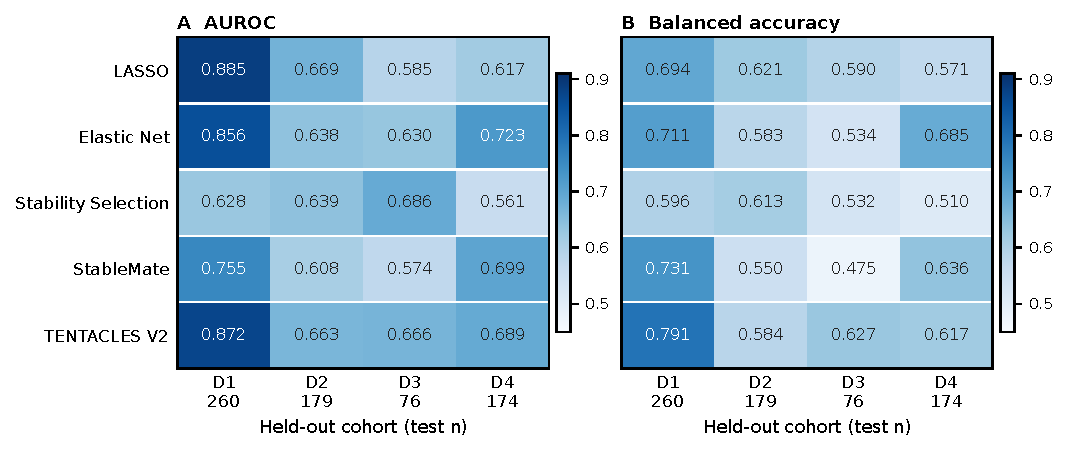
\includegraphics[width=\textwidth]{heldout_metric_heatmaps.pdf}
\caption{External test performance of all five gene-panel selectors, separately for each left-out cohort. Both panels use the same fixed, class-balanced logistic classifier ($C=1$), fitted and scaled on the other three cohorts. Entries show (A) area under the receiver-operating-characteristic curve (AUROC) and (B) balanced accuracy, equal to the mean of CD sensitivity and \emph{Not IBD} specificity at probability threshold 0.5. Cohort sample counts are given below D1--D4; darker cells indicate higher values. The same test patients are used for all methods within each column.}
\label{fig:results_heatmap}
\end{figure*}

Performance depended strongly on the held-out cohort (Fig.~\ref{fig:results_heatmap}). On D1, LASSO attained AUROC 0.885, whereas Stability Selection obtained 0.628. On D3, Stability Selection led with AUROC 0.686; on D4, Elastic Net led with 0.723. TENTACLES was not the best-scoring selector in every test cohort. AUROC and balanced accuracy could also disagree: Stability Selection reached AUROC 0.686 on D3 but balanced accuracy 0.532 at the fixed probability cutoff. The contrast is relevant because CD prevalence varied from 44.7\% in D3 to 83.8\% in D1.

\subsection{TENTACLES consensus-vote sensitivity}
\label{sec:results_tentacles}
The corrected TENTACLES workflow yielded primary six-of-nine consensus panels of 73, 91, 81 and 61 genes (D1--D4). All native exported votes matched these panels and all 689 held-out predictions matched their reported scores. The primary rule gave mean AUROC 0.723 and mean balanced accuracy 0.655. Relaxing the consensus to five votes selected 90--115 genes per fold and reduced mean AUROC to 0.691 (Table~\ref{tab:tentacles_sensitivity}). Six votes performed better on D1, D3 and D4, but not on D2; it should not be described as uniformly superior.

\begin{table}[!t]
\caption{TENTACLES V2 on each held-out cohort: prespecified 6/9-vote primary versus 5/9-vote sensitivity. AUROC intervals are 95\% patient-stratified bootstrap intervals (1,000 resamples), conditional on the fitted six-vote model; they do not quantify variability across new cohorts. BA is balanced accuracy.}
\label{tab:tentacles_sensitivity}
\centering\footnotesize
\setlength{\tabcolsep}{2.9pt}
\renewcommand{\arraystretch}{1.1}
\begin{tabular}{@{}lcccc@{}}
\toprule
Test & 6-vote genes & 6-vote AUROC [95\% CI] & 6-vote BA & 5-vote AUROC\\
\midrule
D1 & 73 & 0.872 [0.821, 0.918] & 0.791 & 0.824\\
D2 & 91 & 0.663 [0.569, 0.753] & 0.584 & 0.666\\
D3 & 81 & 0.666 [0.529, 0.796] & 0.627 & 0.647\\
D4 & 61 & 0.689 [0.608, 0.765] & 0.617 & 0.626\\
\midrule
Mean & 76.5 & 0.723 & 0.655 & 0.691\\
\bottomrule
\end{tabular}
\end{table}

D3 and D4 required documented recoveries of previously saved native fits rather than new fitting runs. D3 lacked XGBoost variable importance; D4 had only four selected cross-validation resamples for XGBoost. Both exceptions concern the model excluded from the prespecified nine-voter consensus. The other nine voters passed the saved orientation and feature-importance checks; native tuning warnings remain and are not erased by the successful downstream evaluation.

\subsection{Gene-panel agreement and size sensitivity}
\label{sec:results_genes}
The relationship between prediction and gene-set agreement was not monotonic (Fig.~\ref{fig:tradeoff}). LASSO and TENTACLES achieved similar mean LOCO Jaccard similarity (0.211 and 0.210), despite selecting on average 282 and 77 genes, respectively (Table~\ref{tab:results_main}). Elastic Net slightly exceeded LASSO's mean AUROC but had a lower mean gene Jaccard (0.115 versus 0.211). StableMate selected an average of 16 genes and had the lowest mean Jaccard (0.033). These values are sensitive to panel size and the shared cohorts in the LOCO training sets.

\begin{figure*}[!t]
\centering
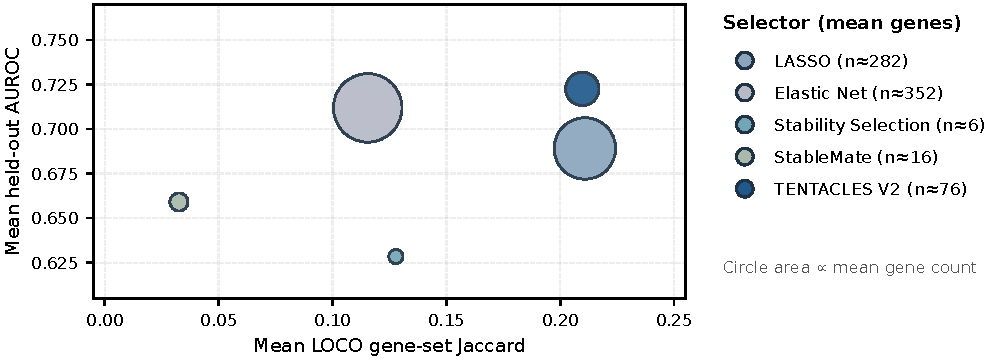
\includegraphics[width=0.92\textwidth]{prediction_vs_agreement.pdf}
\caption{Observed prediction--selection relationship for five methods. Each circle locates the four-cohort mean held-out AUROC versus the mean Jaccard of six pairs of overlapping-training LOCO gene lists. Circle area reflects mean panel size, and the legend identifies each method. The plot is descriptive; selection panel sizes and upstream procedures are not matched.}
\label{fig:tradeoff}
\vspace{1ex}
\begin{minipage}[t]{0.485\textwidth}
\centering
\captionof{table}{Independent-cohort sparse signatures. Gene counts are from models fitted separately within each cohort; mean $\bar J$ covers six patient-disjoint cohort pairs. These gene lists were not used in held-out prediction.}
\label{tab:independent_sizes}
\vspace{0.4ex}
\footnotesize
\setlength{\tabcolsep}{5pt}
\begin{tabular}{@{}lrrrrc@{}}
\toprule
Selector & D1 & D2 & D3 & D4 & $\bar J$\\
\midrule
LASSO & 2523 & 2119 & 1734 & 2623 & 0.164\\
Elastic Net & 2831 & 4025 & 1934 & 2905 & 0.209\\
\bottomrule
\end{tabular}
\end{minipage}\hfill
\begin{minipage}[t]{0.485\textwidth}
\centering
\captionof{table}{Reactome v98 enrichment in four LOCO training panels per method. D1--D4 are counts of pathways passing Benjamini--Hochberg $q<0.05$. $\bar J$ averages nonempty-union pathway-set pairs; n/a indicates all unions empty. Gene-panel sizes differ.}
\label{tab:results_pathways}
\vspace{0.4ex}
\footnotesize
\setlength{\tabcolsep}{4pt}
\begin{tabular}{@{}lccc@{}}
\toprule
Selector & D1/D2/D3/D4 & Folds & $\bar J$\\
\midrule
LASSO & 1/3/4/0 & 3/4 & 0.222\\
Elastic Net & 3/1/4/9 & 4/4 & 0.273\\
Stability Selection & 0/0/0/0 & 0/4 & n/a\\
StableMate & 0/0/0/0 & 0/4 & n/a\\
TENTACLES V2 & 0/11/8/9 & 3/4 & 0.256\\
\bottomrule
\end{tabular}
\end{minipage}
\vspace{2.0ex}
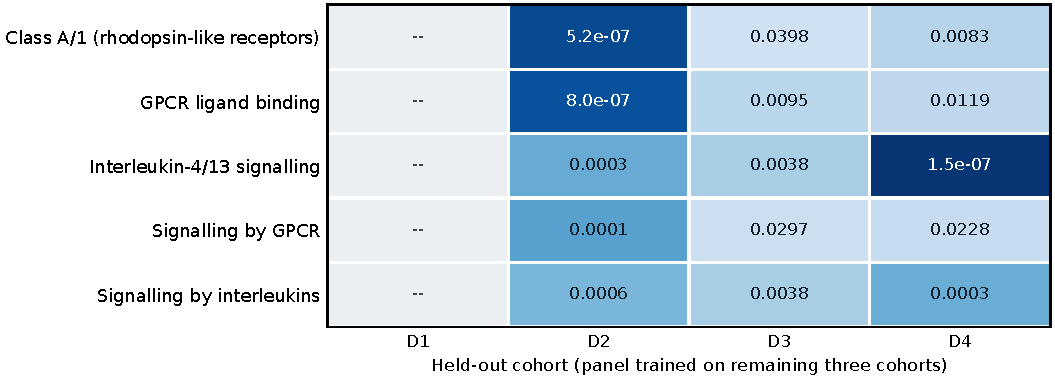
\includegraphics[width=0.88\textwidth]{tentacles_v2_reactome_terms.pdf}
\captionof{figure}{Recurring Reactome v98 terms in the TENTACLES V2 six-vote LOCO panels. Each cell shows the adjusted enrichment $q$ value when $q<0.05$; ``--'' indicates no significant term. These are descriptive overlaps because LOCO training cohorts and gene annotations overlap.}
\label{fig:v2_pathways}
\end{figure*}

Only six genes appeared in all four primary TENTACLES V2 panels: \textit{CLDN18}, \textit{FFAR2}, \textit{MMP3}, \textit{NOS2}, \textit{PAQR5} and \textit{PML}. These are repeated LOCO selections, not independently validated clinical markers. Each LOCO training pair shares two cohorts; consequently the six pairwise Jaccard measurements are dependent rather than six independent replications.

A four-gene, fixed-size sensitivity analysis was possible for LASSO, Elastic Net, Stability Selection and StableMate only: one stability-selection panel contained just four genes. Their respective mean top-four Jaccards were 0.103, 0, 0.103 and 0.048. The corresponding top-ten comparison, available only for LASSO, Elastic Net and StableMate, yielded 0.137, 0.037 and 0.035. TENTACLES V2 supplies genuine vote counts but many equal-count ties, making its top-four ordering arbitrary without a further prespecified rule. Thus the four-method size-matched result cannot be presented as a five-method test. Fixing $K$ also changes the target from agreement of the full selected panel to agreement among a few highest-ranked genes.

To examine gene overlap from patient-disjoint discovery groups, we also fitted LASSO and Elastic Net separately within each cohort. The resulting gene sets were much larger than their LOCO counterparts (Table~\ref{tab:independent_sizes}); mean pairwise Jaccard was 0.164 for LASSO and 0.209 for Elastic Net. Their sizes make these values hard to interpret as evidence of selective, reproducible biomarkers, despite the nonoverlapping patients.


\subsection{Reactome pathway overlap}
\label{sec:results_pathways}
Across the five LOCO panel types, the number of significantly over-represented Reactome pathways varied sharply (Table~\ref{tab:results_pathways}). TENTACLES V2 yielded 0, 11, 8 and 9 significant pathways across D1--D4, with mean pairwise significant-pathway Jaccard 0.256. Elastic Net yielded 3, 1, 4 and 9 pathways ($\bar J=0.273$), and LASSO yielded 1, 3, 4 and 0 ($\bar J=0.222$). No fold of Stability Selection or StableMate produced FDR-significant pathways; their Jaccard similarities are therefore undefined because every compared pathway set is empty, not because the overlap equals zero.


In the V2 panels, interleukin signalling, interleukin-4/interleukin-13 signalling and several G-protein-coupled receptor pathways appeared as significantly enriched terms in D2, D3 and D4 (Fig.~\ref{fig:v2_pathways}). No TENTACLES pathway survived FDR correction in D1. Enrichment reflects over-representation of selected genes against each fold's eligible-gene background, not differential expression, biological causation or independent pathway replication.




